%% LyX 2.0.0 created this file.  For more info, see http://www.lyx.org/.
%% Do not edit unless you really know what you are doing.
\documentclass[english]{article}
\usepackage[T1]{fontenc}
\usepackage[latin9]{inputenc}
\usepackage{graphicx}
\usepackage{babel}
\begin{document}

\title{Assgn4: Notes }

\maketitle

\section*{Notes on GORDIAN}


\section{Set up C}

\[
C_{\mu,\mu}=\sum_{\nu\in N\left(\mu\right)}\frac{2}{p_{\nu}}\left(p_{\nu}-1\right)
\]


\[
C_{\mu,\lambda}=\sum_{\nu\in N\left(\mu\right)\cap N\left(\lambda\right)}-\frac{2}{p_{\nu}}
\]


where, $\mu$ is a \textbf{movable block.} $N\left(\mu\right)$ is
the set of all nets to which $\mu$ is connected.

$p_{\nu}$ is the number of terminals of net $\nu$.


\section{Set up d\_x, d\_y}

\[
dx_{\mu}=\sum_{\nu\in N\left(\mu\right)}\left[\left(p_{\nu}-1\right)\frac{2}{p_{\nu}}\, XPO\left(\mu,\nu\right)-\sum_{\lambda\in MBCB}\frac{2}{p_{\nu}}\, XPO\left(\lambda,\nu\right)-\sum_{\lambda\in FBCB}\frac{2}{p_{\nu}}\, XP\left(\lambda,\nu\right)\right]
\]


where, $\mu$ is a \textbf{movable block, $\lambda$ }could be a movable/fixed
block or a terminal\_NI\textbf{.} $N\left(\mu\right)$ is the set
of all nets to which $\mu$ is connected.

$p_{\nu}$ is the number of terminals of net $\nu$. 

$XPO\left(\mu,\nu\right)$ is the X Pin Offset of the pin connecting
block $\mu$ to the net $\nu$. $XP\left(\lambda,\nu\right)$ is the
X Pin Position of the pin connecting $\lambda$, a fixed block or
terminal\_NI, to the net $\nu$.

MBCB is acronym for {}``Movable Blocks Connected to Block $\mu$
through net $\nu$''

FBCB is acronym for {}``Fixed Blocks Connected to Block $\mu$ through
net $\nu$''

\begin{figure}
\begin{centering}
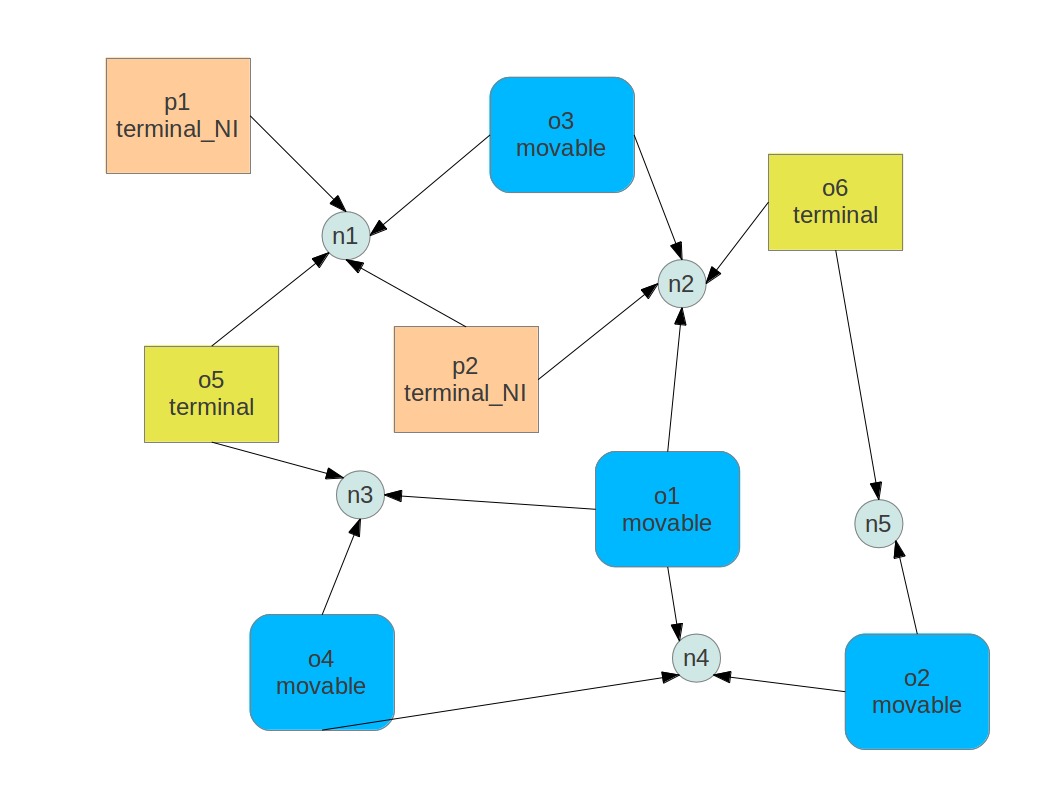
\includegraphics[scale=0.3]{setupC/toy}
\par\end{centering}

\caption{Toy example}


\end{figure}

\end{document}
